\section{Routing Algorithms}
To be able to utilise parking information in order to inform drivers of the real-time states of urban parking spots; whether they be in parking lots or on-street spots. Different algorithms have been proposed by different papers \cite{4}, \cite{6} and \cite{7}.

\subsubsection{Salesman Model}
A well defined algorithm is discussed \cite{6}, that takes into account multiple factors that are of concern. A major problem with working with smart parking systems is to try to deter drivers from arriving at parking spots that have just become occupied. Thus, the analysis that follows will be based on the formula below.

[ C(a,b,t\textsubscript{tot}) = t\textsubscript{ab} + p(t\textsubscript{tot}) * \[\omega\]\textsubscript{b} + [1 - p(t\textsubscript{tot})] * D]

The formula is based loosely on the travelling salesman method. Whereby the aim is to devise a least cost path for a driver to get to a parking spot.

t\textsubscript{ab}: Time required to drive from space a to space b

\[\omega\]\textsubscript{b}: $ Time to walk from space to destination $

D: Time penalty for if space is taken

t\textsubscript{tot}: Time until parking spot is reached

p(t\textsubscript{tot}): Probability that the space is still available

\[\omega\]\textsubscript{b} $ The time to walk to the destination is weighted by p(t\textsubscript{tot}) the probability that the space will still be available. $

Whereas D is weighted by the complement of the probability that the space will not be there.

p(t\textsubscript{tot}) is calculated by an space average life-time (salt) variable. 

Whereby: 

\[ p(t\textsubscript{tot}) = \frac{salt}{t\textsubscript{tot} + salt} \]

The time penalty D may be calculated with the factors of the spaces that the driver has missed, due to destined parking spots being occupied before the driver arrives at it, the time it takes to drive from one spot to another spot (sts) and also the average walk time from all spaces to the destination (wat).

Thus the time penalty can be formulated as:

\[ D = asm * sts + wat \]

This algorithm performs to dynamically allocate a route for a driver through designated parking spot locations.

Other forms discussed in the paper \cite{6} is to cluster parking spaces into areas that the driver may traverse to; to cluster spaces near where the drivers destination is. Since the routing algorithms are to be calculated on the drivers device, by clustering a group of spaces, the load complexity in the calculations will be minimised.

\subsubsection{Reservation-Based Models}
Reservation-based systems have also been researched, whereby drivers are able to buy spaces before parking their cars. A central reservation-based system is discussed \cite{2}. The paper is mainly focused on parking lot infrastructure, thus the parking management system may be easier to handle. It devises a solution whereby drivers communicate directly with parking lots in order to obtain information and to reserve spots within the parking lot.

On the other hand, on-street parking reservation-based systems have also been introduced by CrowdPark \cite{8} and a general on-street crowd-sensing system \cite{9}.

However, crowdsensing applications may be the least expensive to implement. In terms of what this essay is concerned with, simulating crowdsensing through the drivers may be difficult to achieve. Thus a simpler model may be possible through the idea of VANETs.

\subsubsection{VANETs Model}
VANETs, which stands for Vehicular ad-hoc Network, is the idea of ad-hoc network communication between vehicles in real-time. Vehicles are able to communicate with other vehicles in their vicinity. VANETs is of interest to autonomous vehicles as valuable information may be shared within a linear road of autonomous vehicles. For example, the concept of platooning may be encouraged; autonomous vehicles are able to share acceleration or braking information for each instance of a vehicle so that all other vehicles behind are able to adjust accordingly so that vehicles driving along the road are in a train-like manner.

VANET models allow parking information shared from vehicle to vehicle within a vicinity. For example, when a car gives up a parking spot, it may announce as so, so that the information may be propagated to a car nearby looking for a space.

An increasing amount of vehicles are being equipped with on-board wireless communication units in order to facilitate wireless network among cars and their environments \cite{10}. Thus attention should be forwarded to simulate such a network with respect to smart parking functionalities.

In another VANET paper, the proposal brought forward involves a Voronoi diagram in order to dissect the regions of an urban area \cite{11}. 

\begin{figure}[H]
    \centering
    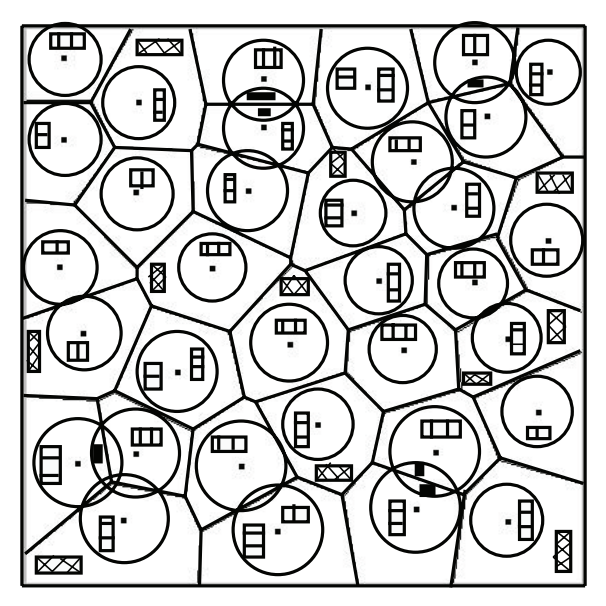
\includegraphics[width=1\linewidth]{./Images/VORONOI.png}
    \caption{Voronoi Model}
    \label{fig:sub1}
\end{figure}

Shown in fig. 1 is a Voronoi model dissecting each section of an urban area. The paper proposes that a road side unit (RSU) should be placed at the center of each individual sector; to handle all the information regarding parking information within its corresponding sector. Thus, each unit handles the occupancy levels of the parking spaces available to their designated areas and the cars with on-board wireless communications units may be able to communicate with each sector that it traverses through.

Although, the drawbacks with this type of implementation would be the cost, as the additional RSUs need to be deployed as well as parking sensors that monitor the parking spaces. This may be necessary for a VANET based system, however unlikely within an urban setting, there may be times where a vehicle is isolated from any nearby networks thus the lack of information for it would render it impossible to receive any type of information.

Furthermore, introduction of a VANET based system would also include distributed system models which have been researched much more thoroughly in terms of computer networks.

\subsubsection{Demand Based Models}
Alternatively, another form of parking space distributions and in turn, routing mechanisms for drivers is to offer a demand based distribution of parking spaces.

SFPark \cite{12} is a pilot project for smart parking, utilising parking sensors installed into a selected amount of on-street parking spaces. the uniqueness in this system is that it tries to keep around 10-15\% of parking spaces free on a street or block. Using a demand based pricing model, it increases the price for street parking spots if the street is near 85-90\% occupancy. Vice versa, if the street is 85-90\% free, then the charges will be low. This is to ensure that the variance of parking spaces available are distributed among the streets. The price rate factors in the time of day, and if any events are currently taking place in the vicinity of the parking locations.

This model is also of interest to be included into the simulation.

\begin{table}[H]
\centering
\resizebox{\textwidth}{!}{%
    \begin{tabular}{@{}|p{3cm}|p{3cm}p{3cm}p{3cm}p{3cm}|@{}}
    \toprule
    Algorithm & Exact-Approach & Cluster Approach & Live Approach & ParkAssistant\\ \midrule
    Time Complexity & $\mathcal{O}(n\textsuperscript{3}T2\textsuperscript{n})$, where n = no. of parking spaces, T = time of longest trip & $\mathcal{O}(n\textsuperscript{3}T2\textsuperscript{n})$, where n = no. of clusters, T = time of longest trip & $\mathcal{O}(n*m)$, where n = number of clusters, m = number of pre-existing spaces & N/A\\ \hline
    
    Dissemination Protocol & On-board calculations attainable from sources & On-board calculations attainable from sources & Near vehicular communications & None, data obtained through central system \\ \hline
    
    Parking Spaces Scope & All available spaces that match drivers' destination criteria & Only takes into account clustered areas that match driver’s destination criteria & Nearby spaces only & All that match drivers criteria\\ \hline
    
    Algorithms Involved & TSA Algorithm & K-medoids, Quality Threshold Clustering & Update system, re-calibration of trajectory algorithm & Algorithm proposed in paper\\ \hline
    
    Parking Allocation Tendencies & No tendencies & Tendency to allocate clustered spaces that match best & Tendency to point drivers to high density parking areas (as algorithm is based on scoring function) & No tendencies \\ \hline
    
    Parking Data & Sensed Data & Sensed Data & Sensed Data & Uncertain Data \\ \bottomrule
    \end{tabular}%
}
\end{table}
